%%%%%%%%%%%%%%%%%%%%%%%%%%%%%%%%%%%%%%%%%
% SLIIT Metropolitan Campus
% Enterprise Software Analysis & Design
% SE5060: Exercise 11
% Version 1.0 (2020-10-23)
%
% Authors:
% Pradeep (sanjayangp@gmail.com)

%
% License:
% CC BY-NC-SA 3.0 (http://creativecommons.org/licenses/by-nc-sa/3.0/)
% 
%%%%%%%%%%%%%%%%%%%%%%%%%%%%%%%%%%%%%%%%%

%----------------------------------------------------------------------------------------
%	PACKAGES AND OTHER DOCUMENT CONFIGURATIONS
%----------------------------------------------------------------------------------------

\documentclass[12pt]{scrartcl} % Font size

\usepackage{amsmath, amsfonts, amsthm} % Math packages

\usepackage{listings} % Code listings, with syntax highlighting

\usepackage[english]{babel} % English language hyphenation

\usepackage{graphicx} % Required for inserting images
\graphicspath{{Figures/}{./}} % Specifies where to look for included images (trailing slash required)

\usepackage{booktabs} % Required for better horizontal rules in tables
\usepackage[shortlabels]{enumitem}
\usepackage{float}


\numberwithin{equation}{section} % Number equations within sections (i.e. 1.1, 1.2, 2.1, 2.2 instead of 1, 2, 3, 4)
\numberwithin{figure}{section} % Number figures within sections (i.e. 1.1, 1.2, 2.1, 2.2 instead of 1, 2, 3, 4)
\numberwithin{table}{section} % Number tables within sections (i.e. 1.1, 1.2, 2.1, 2.2 instead of 1, 2, 3, 4)

\setlength\parindent{0pt} % Removes all indentation from paragraphs

\usepackage{enumitem} % Required for list customisation
\setlist{noitemsep} % No spacing between list items

%----------------------------------------------------------------------------------------
%	DOCUMENT MARGINS
%----------------------------------------------------------------------------------------

\usepackage{geometry} % Required for adjusting page dimensions and margins

\geometry{
	paper=a4paper, % Paper size, change to letterpaper for US letter size
	top=2.5cm, % Top margin
	bottom=3cm, % Bottom margin
	left=3cm, % Left margin
	right=3cm, % Right margin
	headheight=0.75cm, % Header height
	footskip=1.5cm, % Space from the bottom margin to the baseline of the footer
	headsep=0.75cm, % Space from the top margin to the baseline of the header
	%showframe, % Uncomment to show how the type block is set on the page
}

%----------------------------------------------------------------------------------------
%	FONTS
%----------------------------------------------------------------------------------------

\usepackage[utf8]{inputenc} % Required for inputting international characters
\usepackage[T1]{fontenc} % Use 8-bit encoding

\usepackage{times} % Use the Adobe Utopia font for the document

%----------------------------------------------------------------------------------------
%	SECTION TITLES
%----------------------------------------------------------------------------------------

\usepackage{sectsty} % Allows customising section commands

\sectionfont{\vspace{6pt}\centering\normalfont\scshape} % \section{} styling
\subsectionfont{\normalfont\bfseries} % \subsection{} styling
\subsubsectionfont{\normalfont\itshape} % \subsubsection{} styling
\paragraphfont{\normalfont\scshape} % \paragraph{} styling

%----------------------------------------------------------------------------------------
%	HEADERS AND FOOTERS
%----------------------------------------------------------------------------------------

\usepackage{scrlayer-scrpage} % Required for customising headers and footers

\ohead*{} % Right header
\ihead*{} % Left header
\chead*{} % Centre header

\ofoot*{} % Right footer
\ifoot*{} % Left footer
\cfoot*{\pagemark} % Centre footer
 % Include the file specifying the document structure and custom commands

%----------------------------------------------------------------------------------------
%	TITLE SECTION
%----------------------------------------------------------------------------------------

\title{	
	\normalfont\normalsize
	\textsc{Master of Science in Information Technology Specializing in Enterprise Applications Development}\\
	\textsc{SLIIT Metropolitan Campus}\\
	\textsc{BOC Merchant Tower, No \#28, St Michae\rq{}s Road,}\\
	\textsc{Colombo 03, Sri Lanka}\\
	\vspace{25pt} % Whitespace
	\rule{\linewidth}{0.5pt}\\ % Thin top horizontal rule
	\vspace{20pt} % Whitespace
	{\huge Enterprise Software Analysis \& Design}\\
	\textsc{SE5060: Exercise 11}\\
	\vspace{12pt} % Whitespace
	\rule{\linewidth}{2pt}\\ % Thick bottom horizontal rule
	\vspace{12pt} % Whitespace
}

\author{\LARGE N. G. Pradeep Sanjaya\\
	\small{MS20921576}
} % Your name

\date{\normalsize\today} % Today's date (\today) or a custom date

\begin{document}

\maketitle % Print the title

\newpage
\section*{Answer}
Github - https://github.com/pradeep-sanjaya/ead-esad-exercise11

\subsection*{Classes}


\textbf{FilterTest.java}
\lstset{language=Java}
\begin{lstlisting}[frame=single]
package com.sliit;

public class FilterTest {
  public static void main(String[] args) {
    Filter filter = new AuthenticationFilter(
      new DebuggingFilter(
        new InputValidationFilter(null)
      )
    );
    filter.execute();

    System.out.println();
    new AuthenticationFilter(new DebuggingFilter(null)).execute();

    System.out.println();
    new AuthenticationFilter(null).execute();

    System.out.println();
    new InputValidationFilter(new DebuggingFilter(
      new AuthenticationFilter(null))
    ).execute();
  }
}
\end{lstlisting}


\textbf{Filter.java}
\lstset{language=Java}
\begin{lstlisting}[frame=single]
package com.sliit;

public interface Filter {
  void execute();
}
\end{lstlisting}


\textbf{AbstractFilter.java}
\lstset{language=Java}
\begin{lstlisting}[frame=single]
package com.sliit;

public class AbstractFilter implements Filter {
  Filter filter;

  public AbstractFilter(Filter filter) {
    this.filter = filter;
  }

  @Override
  public void execute() {
    if (filter != null) {
      filter.execute();
    }
  }
}
\end{lstlisting}


\textbf{AuthenticationFilter.java}
\lstset{language=Java}
\begin{lstlisting}[frame=single]
package com.sliit;

public class AuthenticationFilter extends AbstractFilter {

  public AuthenticationFilter(Filter filter) {
    super(filter);
  }

  @Override
  public void execute() {
    System.out.println("Authentication Filter");
    super.execute();
  }
}
\end{lstlisting}

\textbf{DebuggingFilter.java}
\lstset{language=Java}
\begin{lstlisting}[frame=single]
package com.sliit;

public class DebuggingFilter extends AbstractFilter {

  public DebuggingFilter(Filter filter) {
    super(filter);
  }

  @Override
  public void execute() {
    System.out.println("Debugging Filter");
    super.execute();
  }
}
\end{lstlisting}


\textbf{Chicken.java}
\lstset{language=Java}
\begin{lstlisting}[frame=single]
package com.sliit;

public class InputValidationFilter extends AbstractFilter {

  public InputValidationFilter(Filter filter) {
    super(filter);
  }

  @Override
  public void execute() {
    System.out.println("Input Validation Filter");
    super.execute();
  }
}
\end{lstlisting}

\subsection*{Screenshots}
\begin{center}
	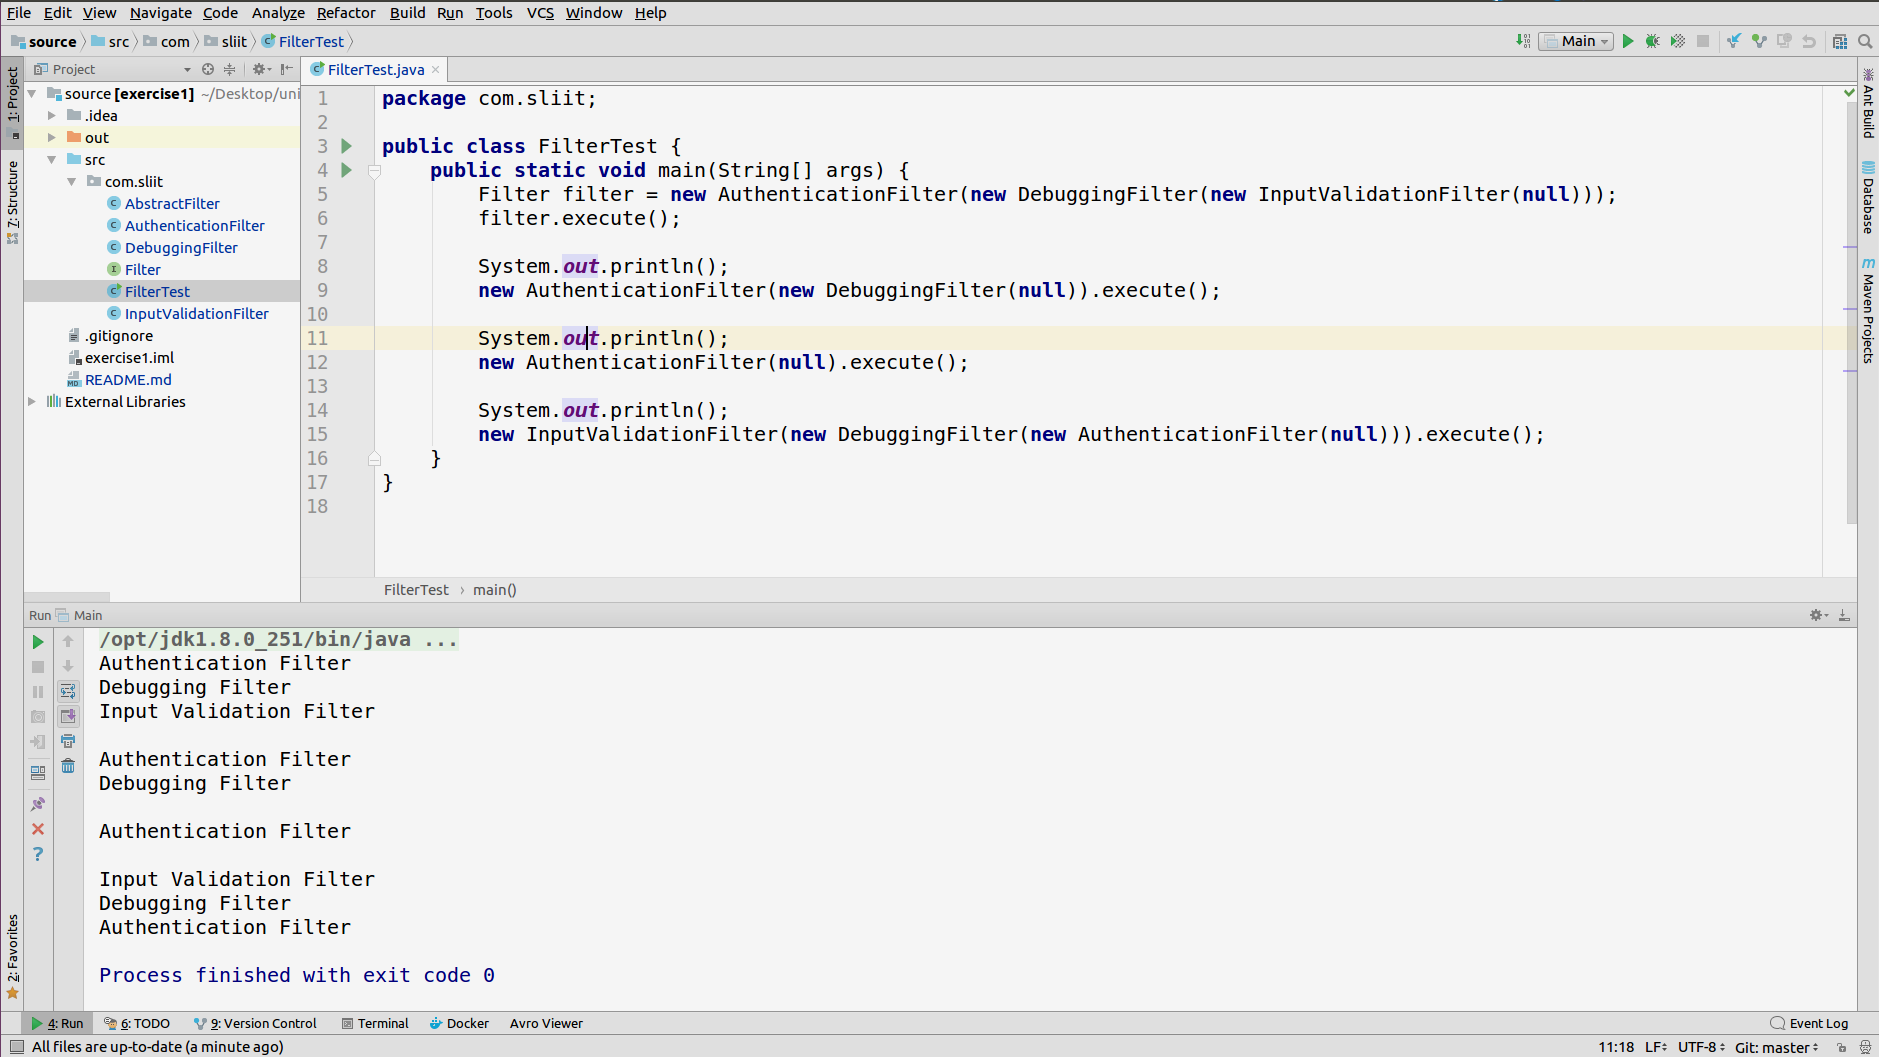
\includegraphics[width=1.0\columnwidth]{./figures/01.png}
	\captionof{figure}{Solution}\label{Solution}%
\end{center}


\pagebreak
\newpage
\begin{thebibliography}{00}
	\raggedright
    \bibitem{b1} Samarathunge, U. (2020) Lecture-04 - Presentation Layer Patterns.pptx
\end{thebibliography}


\end{document}
